\section{AC: Activity Clustering}
\label{sec:clustering:ac}

Initial clusters provided by $SA^3$ are expanded in this step, using context knowledge and time-based metrics for action aggregation. The inputs of the $AC$ algorithm are the context knowledge file (see Section \ref{sec:approach:solution} and specially Figure \ref{fig-context-json}) and the partially annotated dataset returned by $SA^3$ (see Figure \ref{fig-partially-annotated}). The output of $SA^3$ is interpreted as the initialisation of the clustering process in the activity space spanned by location, type and time axis. $SA^3$ has been designed to provide the number of clusters in the dataset, their semantic label and their centroids in the time axis. Having this initialisation, $AC$ is the responsible of analysing all actions considering the three dimensions of the activity space and deciding which actions are aggregated to the initial clusters provided by $SA^3$.

Assume Figure \ref{fig-initial-clusters} shows the output of $SA^3$ for a concrete sequence of actions. For simplicity, only the time axis is shown in the figure. Dashes represent time intervals without any action. Circles represent actions that are in one or more IAMs. Notice that two circles do not necessarily have to be the same action. The only property they have is that a circle action is in at least one of the IAMs of the context knowledge file. Crosses, on the other hand, are actions that are not included in any IAM. Once again, two crosses do not have to represent the same action. 

\begin{figure}[htbp]%[!t]
\centering
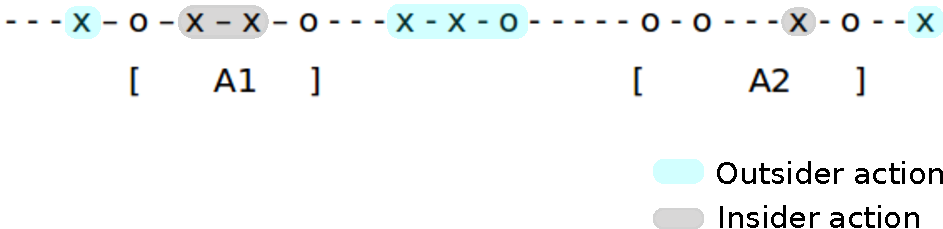
\includegraphics[width=\textwidth]{clustering_ex_complete.pdf}
    \caption{Output of $SA^3$ for a concrete sequence of actions, where outsider and insider actions are identified.}
    \label{fig-initial-clusters}
\end{figure}

Figure \ref{fig-initial-clusters} shows that $SA^3$ detects activities $A_1$ and $A_2$ in that sequence of actions. As stated in Section \ref{sec:clustering:sa3} only actions that are in the IAM of the detected activity can be really considered part of that activity, i.e. only circles that are inside activities $A_1$ and $A_2$ are labelled with corresponding activity labels. 

Given that action classification, two new definitions can be assumed:

\begin{defn}[Insider action]
\label{def-insider}
 Every action that is inside initial clusters provided by $SA^3$ but is not in their IAMs is considered an \textit{insider action} or \textit{insider}, in short.
\end{defn}

\begin{defn}[Outsider action]
\label{def-outsider}
 Every action out of initial clusters provided by $SA^3$ is an \textit{outsider action} or \textit{outsider}, in short.
\end{defn}

Due to single-user single-activity scenario constraint (constraint \ref{cons-single}), an insider may pertain to its wrapping activity or to none, i.e. it has been produced by noise or user erratic behaviour. There is no chance for an insider to pertain to an activity other than its wrapping activity because such an assumption would imply the existence of interleaved activities. The situation for outsiders is different since an outsider can pertain to its previous activity, next activity or to none. 

The inherent difference between insiders and outsiders demands a different treatment for both cases. $AC$ first treats all insider actions and afterwards computes all outsiders using different approaches.

\subsection{Insider actions}
To decide whether an insider has to be added to its wrapping activity, a \textit{compatibility function} between an activity and an action is defined. The compatibility function is a boolean function that captures whether an insider action has been executed in the same location as the activity and its purpose is coherent with the activity type:

\begin{equation}
\label{eq-comp}
 Comp(A, a) = Loc(A, a) \wedge Type(A, a)
\end{equation}

\noindent where $A$ is an activity and $a$ is an action. $Loc(A, a)$ is the location compatibility between an activity and an action, defined as in Section \ref{subsec:clustering:sa3:find}. The location of the concrete activity $A$ is inferred using the same process as in $SA^3$, i.e. the common location of the actions pertaining to the IAM of the activity is set to be the location of the activity. $Loc(A, a)$ returns whether the inferred location for action $a$ is the same as the inferred location for activity $A$. On the other hand, $Type(A, a)$ is the type compatibility between an activity and an action. Action type is inferred from the object used to execute the action. Every object in the context knowledge has a list of types. Activity type is unique and it is also retrieved from the context knowledge file. So $Type(A, a)$ is calculated as the intersection between the list of types of the action $a$ and the type of the activity $A$. If the intersection is empty, the action and the activity are not type compatible.

Hence an insider action $a$ will only be aggregated to its wrapping activity $A$, if $Comp(A, a) = True$, i.e. the insider has been executed in the same location of the activity, and its purpose is compatible with the activity type. If $Comp(A, a) = False$, the insider will be labelled with the None label, which means that it is not part of any activity.

\subsection{Outsider actions}
As an outsider can be aggregated to its previous or next activity, first of all the algorithm checks the feasibility of both options, defining another boolean function called \textit{candidate function}:

\begin{equation}
\label{eq-candidate}
 Cand(A, a) = Comp(A, a) \wedge InRange(A, a)
\end{equation}

\noindent $Comp(A, a)$ has already been defined in equation \ref{eq-comp}, so the candidate function also takes into account location and type. $InRange$ function is another boolean function that captures time feasibility. Thus the candidate function states that an activity $A$ is a candidate activity for action $a$, if they are compatible ($Comp(A, a) = True$) and in range ($InRange(A, a) = True$). 

As commented above, $InRange$ function has been defined to capture the time feasibility. For example, if an action has been executed two hours before an activity whose estimated duration is three minutes, the action should not be aggregated to that activity, since it is almost impossible for the action to be related with the activity. This reasoning can be implemented in a boolean function using time distance and activity duration.

To capture time feasibility, the duration given by the expert in an IAM is interpreted as the standard deviation for concrete executions of that activity, i.e. the vast majority of the activities executed by any user, will lie inside the time area limited by the duration. This can be seen in Figure \ref{fig-in-range}. So time distances among actions pertaining to a concrete activity are modelled by a Gaussian distribution, where the duration estimation given by the expert for that activity is the standard deviation. A Gaussian distribution has been selected, because it captures perfectly the idea of activity duration as a time estimation where the majority of executions of that activity occur. The probability for actions of an activity to lie in the area limited by the duration estimation is very high and gets lower as it gets further from that duration.

Nevertheless, due to human behaviour variations, there will be some executions whose duration is outside the standard deviation. To capture those executions, $InRange$ function considers all the actions lying inside $k$ standard deviations. For the experiments run in this dissertation $k=2$ has been set, but the value can be adjusted depending on the area which is desired to cover. For a concrete activity execution, the mean of the activity is calculated as the centre of the detected start and end of the activity, as given by $SA^3$. Using this mean calculation, duration estimation given in the context knowledge is the standard deviation of the Guassian distribution for action time distances. Hence, in the case depicted in Figure \ref{fig-in-range}, where Gaussian distributions are calculated as described, the outsider action represented with a star is in range with activities $A_1$ and $A_2$ for $k=2$.

\begin{figure}[htbp]%[!t]
\centering
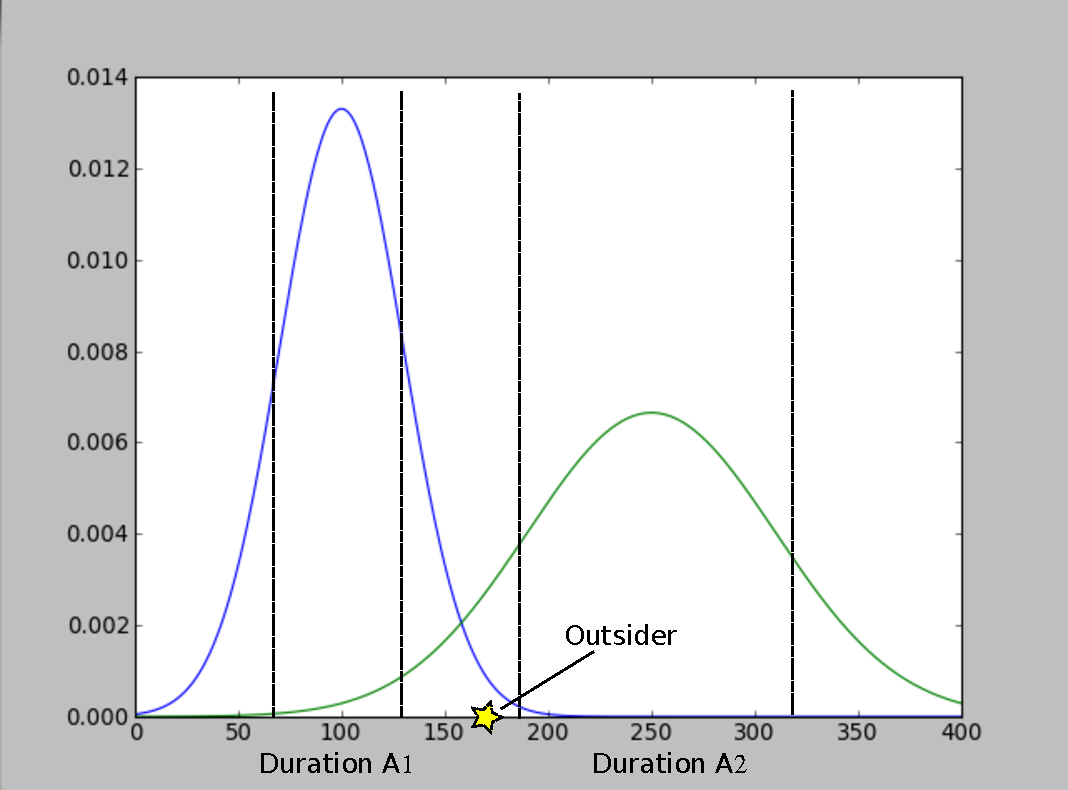
\includegraphics[width=\textwidth]{in_range_criterion.pdf}
    \caption{Gaussian distributions of activity durations for activities $A_1$ and $A_2$. Vertical lines show the standard deviation and the star represents an outsider action.}
    \label{fig-in-range}
\end{figure}

In consequence, using the candidate function, the following cases can be faced for an outsider action $a$ and surrounding activities $A_1$ and $A_2$:

\begin{enumerate}
 \item $Cand(A_1, a) = Cand(A_2, a) = False \rightarrow$ $a$ is noise (None label)
 \item $Cand(A_1, a) = True \wedge Cand(A_2, a) = False \rightarrow$ aggregate $a$ to $A_1$
 \item $Cand(A_1, a) = False \wedge Cand(A_2, a) = True \rightarrow$ aggregate $a$ to $A_2$
 \item $Cand(A_1, a) = Cand(A_2, a) = True \rightarrow$ need of a new heuristic
\end{enumerate}

The first three cases provide a clear classification for an outsider. The candidate function determines unambiguously the label for action $a$. But for the fourth case, where previous and next activities are both candidate activities, a new heuristic has to be defined. There is no more information in the context knowledge than the location and type information to relate outsider actions to activities, thus context knowledge cannot be used to decide between activities $A_1$ and $A_2$. Hence a new heuristic is defined stating that an outsider action $a$ will be aggregated to the time closest activity:

\begin{equation}
 min\{\Delta_t(A_1, a), \Delta_t(A_2, a)\}
\end{equation}

To implement this heuristic, a definition for $\Delta_t(A, a)$, the time distance between an activity and an action, is needed. As an activity has a duration and an action is described by a time instant, three time metrics are proposed:

\begin{enumerate}
 \item Simple time distance: the distance between the centre of the activity as given by $SA^3$ and the action time coordinate.
 \begin{equation}
 \label{eq-t1}
  \Delta_t(A, a) = | C_A - t_a |,\ where \ C_A = \frac{t_{end} ^{SA^3} - t_{start} ^{SA^3}}{2}
 \end{equation}
 \item Normalised time distance: simple time distance normalised by the duration of the activity as given by the expert. This time metric, as opposed to the simple time distance, treats equally all activities regardless their duration. Notice that duration given by the expert is used rather than the duration detected by $SA^3$, since $SA^3$ may give varying durations depending on the order of executed actions that pertain to the IAM of the detected activity. Hence, the duration given by $SA^3$ cannot be a good reference. But notice also that to calculate the centre of the activity, the output of $SA^3$ is used. In this case, this information is the only one that allows calculating the centre. So the duration given by the expert is projected symmetrically around the centre calculated from $SA^3$:
 \begin{equation}
 \label{eq-t2}
  \Delta_t(A, a) = \frac{| C_A - t_a |}{Duration_A} ,\ where \ C_A = \frac{t_{end} ^{SA^3} - t_{start} ^{SA^3}}{2}
 \end{equation}
 \item Dynamic centre normalised time distance: only used for previous activity, it dynamically calculates the centre of the activity depending on already aggregated actions.
 \begin{equation}
 \label{eq-t3}
  \Delta_t(A, a) = \frac{| C_A - t_a |}{Duration_A} ,\ where \ C_A = \frac{t_{start} ^{AC} + Duration_A}{2}
 \end{equation}
\end{enumerate}

Let us explain the third time distance in detail. Activity start and end times provided by $SA^3$ are not generally trustful, since they depend on what actions are in the IAM of the detected activity and on the order of executions of those actions by the user. Imagine that $IAM(A)=\{a, b\}$ and that the action sequence processed by $SA^3$ is $S=\{d, b, a, c\}$. Assume that sequence $S$ is the action sequence performed by the user for activity $A$. $SA^3$ will detect that activity $A$ is being performed in sequence $S$, but it will only label actions $b$ and $a$ as pertaining to the activity. $SA^3$ does not have any information to know whether actions $d$ and $c$ pertain to activity $A$. So the start time of activity $A$ for $SA^3$ will be the time-stamp associated to action $b$ and not to action $d$. The same happens for the activity end time.

Nevertheless, while executing the $AC$ algorithm, starting times of activities can be estimated better, but with some limitations. In the previous example, as outsiders in $AC$ are treated in time order for convenience, when treating outsider $c$, its previous activity's previous actions have already been treated (in this case, action $d$). $AC$ has already determined that action $d$ pertains to activity $A$. This means that the start of that previous activity $A$ has been fixed and it is different from the start time provided by $SA^3$ ($t_{start} ^{AC} \neq t_{start} ^{SA^3}$).

In contrast with time metrics 1 and 2, where activity start and end were given by $SA^3$ and activity duration was assumed to be located symmetrically around the centre of the activity, the third time metric uses the start time of the previous activity as found by $AC$. Afterwards, the centre of the activity is calculated projecting the duration from the starting point. This makes previous activity treatment more accurate. However, notice that the same approach cannot be applied to the next activity, since it has not been treated yet. The estimation given by $SA^3$ cannot be improved, because surrounding activities have not been treated when action $c$ is being analysed. Hence, the best guess is to keep using start and end times provided by $SA^3$.

\subsection{The complete AC algorithm}
\label{subsec:clustering:complete-ac}

To sum up, the $AC$ algorithm takes the results of $SA^3$ as the initialisation step. First, it treats insiders for all the activities detected by $SA^3$, using the compatibility function (equation \ref{eq-comp}). Afterwards, it treats outsiders in time order, using the candidate function (equation \ref{eq-candidate}) and defined three time metrics (equations \ref{eq-t1}, \ref{eq-t2} and \ref{eq-t3}). The complete algorithm is depicted as pseudo-code in Algorithm \ref{alg:ac}.

\begin{algorithm}
 \caption{$AC$ algorithm for activity clustering}
 \label{alg:ac}
 \begin{algorithmic}
 \REQUIRE partially\_annotated\_dataset, context\_knowledge
 \ENSURE fully\_annotated\_dataset, activity\_clusters
 \STATE $fully\_annotated\_dataset \leftarrow createDataset(partially\_annotated\_dataset)$
 \STATE $insiders \leftarrow obtainInsiders(partially\_annotated\_dataset)$
 \STATE $outsiders \leftarrow obtainOutsiders(partially\_annotated\_dataset)$ 
 \FORALL{$action \in insiders$}
  \STATE $activity \leftarrow obtainWrappingActivity(action, partially\_annotated\_dataset)$
  \IF{$Comp(activity, action, context\_knowledge)$}
    \STATE $label(a, activity, fully\_annotated\_dataset)$
  \ELSE
    \STATE $label(a, None, fully\_annotated\_dataset)$
  \ENDIF
 \ENDFOR 
 \FORALL{$action \in outsiders$}  
  \STATE $previous\_activity \leftarrow obtainPreviousActivity(action, partially\_annotated\_dataset)$
  \STATE $next\_activity \leftarrow obtainNextActivity(action, partially\_annotated\_dataset)$
  \STATE $Prev \leftarrow Cand(action, previous\_activity, context\_knowledge)$
  \STATE $Next \leftarrow Cand(action, next\_activity, context\_knowledge)$
  \IF{$\neg Prev \wedge \neg Next$}
    \STATE $label(a, None, fully\_annotated\_dataset)$
  \ELSIF{$Prev \wedge \neg Next$}
    \STATE $label(a, previous\_activity, fully\_annotated\_dataset)$
  \ELSIF{$\neg Prev \wedge Next$}
    \STATE $label(a, next\_activity, fully\_annotated\_dataset)$
  \ELSIF{$Prev \wedge Next$}
    \STATE $// \text{Use time metrics}$
    \STATE $prev\_dist \leftarrow timeDist(action, previous\_activity, time\_metric)$
    \STATE $next\_dist \leftarrow timeDist(action, next\_activity, time\_metric)$
    \IF{$prev\_dist \leq next\_dist$}
      \STATE $label(a, previous\_activity, fully\_annotated\_dataset)$
    \ELSE
      \STATE $label(a, next\_activity, fully\_annotated\_dataset)$
    \ENDIF
  \ENDIF  
 \ENDFOR
 \STATE $activity\_clusters \leftarrow createClusters(fully\_annotated\_dataset)$
 \RETURN $fully\_annotated\_dataset, activity\_clusters$
 \end{algorithmic}
\end{algorithm}

The algorithm returns two files: (i) a fully labelled sensor activation dataset, which is formatted in a CSV file in the current implementation, and (ii) a list of clusters, which has been implemented through a \textit{Json} file. Additionally, that file contains: (i) the frequency of each activity cluster, (ii) duration statistics (mean and standard deviation), (ii) frequencies of used objects and actions and (iii) frequencies of locations per activity. 

An example of the fully annotated dataset can be seen in Figure \ref{fig-fully-annotated}. $AC$ takes the partially annotated dataset generated by $SA^3$ and adds two new columns: the label assigned by $AC$ and the start and end tags for activities. Figure \ref{fig-fully-annotated} is taken from a real experiment and shows very well the difference between $SA^3$ and $AC$. The action sequence depicted shows a particular execution of the MakePasta activity, where due to sensor errors, a \textit{rcontrolSens} activation occurred. It can be seen how $SA^3$ detects that a MakePasta activity is being performed in the action sequence. But activity start and end times differ substantially from the real ones. However, $AC$ detects perfectly activity start and end times, using the outsider action treatment process. And for the insider action \textit{hasRemoteControl}, $AC$ assigns a None label, since the action is not type compatible with the activity. So in this case, $AC$ completes its work perfectly, assigning the appropriate labels to every action and enhancing the results obtained by $SA^3$.

\begin{figure}[htbp]
\begin{scriptsize}
\begin{lstlisting}
2014-05-23 13:34:09.590934,storeSens,openStore,None,,MakePasta,start
2014-05-23 13:34:15.976283,potSens,useCookingUtensil,MakePasta,start,MakePasta,
2014-05-23 13:34:35.067066,ktapSens,turnOnTap,MakePasta,,MakePasta,
2014-05-23 13:35:01.608632,cookerSens,useCookingAppliance,MakePasta,,MakePasta,
2014-05-23 13:35:59.858079,rcontrolSens,hasRemoteControl,MakePasta,,None,
2014-05-23 13:36:15.475288,macaroniSens,hasPasta,MakePasta,end,MakePasta,
2014-05-23 13:45:15.485760,drainerSens,useCookingUtensil,None,,MakePasta,
2014-05-23 13:45:54.969772,fridgeSens,openFridge,None,,MakePasta,
2014-05-23 13:46:00.132993,baconSens,hasBacon,None,,MakePasta,
2014-05-23 13:46:05.764809,creamSens,hasCream,None,,MakePasta,end
\end{lstlisting}
\end{scriptsize}
\caption{Example of a fully annotated dataset, one of the outputs of the $AC$ algorithm.}
\label{fig-fully-annotated}
\end{figure}

An example of the activity clusters file has already been shown in Figure \ref{fig-clusters-file}. As it can be seen in the figure, several concepts per activity are stored in the file:

\begin{enumerate}
 \item Locations: a list of different locations where the activity has been performed with occurrence frequencies. Locations are obtained using activity location inference.
 \item Actions: a list of actions executed by the user to perform the activity with associated occurrence frequencies.
 \item Patterns: patterns refers to different action sequences performed by the user for the activity, i.e. the activity clusters detected by the clustering process. Every detected cluster has its occurrence frequency. 
 \item Objects: a list of objects used by the user while performing the activity. Once again, every object has its occurrence frequency.
 \item Occurrences: the total number of instances of the activity captured by the clustering process, which has to be equal to the sum of all the occurrences of patterns. 
 \item Duration: the mean duration of the detected instances of the activity and the standard deviation, both in seconds.
\end{enumerate}

This information will be used by the Activity Model Learner ($AML$) algorithm to learn EAMs from the clusters extracted by the clustering process. Additionally, the information stored in the activity clusters file may be very useful to domain experts, since they may be able to analyse how activities are carried out by different users in terms of the executed actions, used objects, different sequences of actions and duration. The potential applications of such information, specially considering that it can be updated periodically to monitor the evolution of the user, is out of the scope of this dissertation, but it can open the doors to detect cognitive impairment and its evolution, inappropriate behaviour or user bad habits. 